\chapter{Proof-of-concept}
\label{ch:Proof-of-concept}

In deze proof-of-concept zal er onderzocht worden als een PWA kan voldoen aan het verwachtingspatroon van een gebruiker op een native applicatie.

Er zal een applicatie ontwikkeld worden waarbij een aangemelde gebruiker een  andere persoon zal kunnen uitnodigen om een video gesprek te hebben. 

 \section{Analyse}

	 \subsection{Rollen}
	 
		 \subsubsection{Gebruiker}
			Een persoon die de toepassing gebruikt, deze persoon hoeft niet aangemeld te zijn.
		 
		 \subsubsection{Aangemelde gebruiker}
		 	Dit is een gebruiker die reeds een account heeft op de toepassen en die aangemeld is.
	 
	 \subsection{Functionele requirements}
	 	\subsubsection{Authenticatie}
		 	\begin{itemize}
			 	\item Als een gebruiker wil ik me kunnen registreren met externe platformen (facebook, google, ...) zodat ik minder wachtwoorden hoef te onthouden.
			 	\item Als een aangemelde gebruiker wil ik aangemeld blijven als ik de applicatie sluit zodat ik tijd bespaar door niet niet bij elk gebruik te moeten aanmelden.
		 	\end{itemize}
		 	
		 \subsubsection{Bellen}
			  \begin{itemize}
			   	\item Als een aangemelde gebruiker wil ik een 'room' aanmaken waar ik een video-gesprek kan starten zodat ik in contact kan blijven met iemand waar ik niet fysiek bij kan zijn.
			   	\item Als een aangemelde gebruiker wil ik eenvoudig een link kunnen kopiëren naar mijn room zodat ik deze kan delen met iemand.
			   	\item Als een aangemelde gebruiker wil ik mijn 'rooms' kunnen beheren.
			   	\item Als een aangemelde gebruiker wil ik een notificatie ontvangen als iemand in mijn 'room' komt.
			  \end{itemize}
	 	
	 	\subsubsection{Gebeld worden}
	 	 \begin{itemize}
				\item Als een gebruiker wil ik, als ik een link van een room ontvang, eenvoudig deelnemen aan een videogesprek.
	 	 \end{itemize}
	
		\subsubsection{Algemeen}
	 		\begin{itemize}
	 			\item Als een gebruiker wil een de toepassing toevoegen aan het startscherm van mijn toestel zodat ik deze snel kan openen.
	 			\item Als een aangemelde gebruiker wil ik de applicatie kunnen openen zonder internetverbinding zodat ik mijn overal en altijd mijn rooms kan bekijken.
			\end{itemize}
	 
	\subsection{niet-functionele requirements}
		\begin{itemize}
			\item Als een gebruiker wil ik een video-gesprek kunnen hebben met een zo laag mogelijke vertraging zodat ik geen problemen heb met communiceren.
			\item Als een gebruiker wil ik video-gesprekken voeren op een veilige manier zodat niemand informatie kan achterhalen die ik niet publiek wou maken.
		\end{itemize} 
		


\section{Design}
		\subsection{Mockup}
			https://medium.com/@BuildMySite1/the-what-why-and-how-of-mockups-4799eb115140
			
			Voor er een design gemaakt werd, werden er Mockups opgesteld.
			Aan de hand van deze mockups met weinig detail, kon er snel gestart worden met het ontwikkelen van de functionaliteiten. 
			\begin{figure}[H]
				\centering
				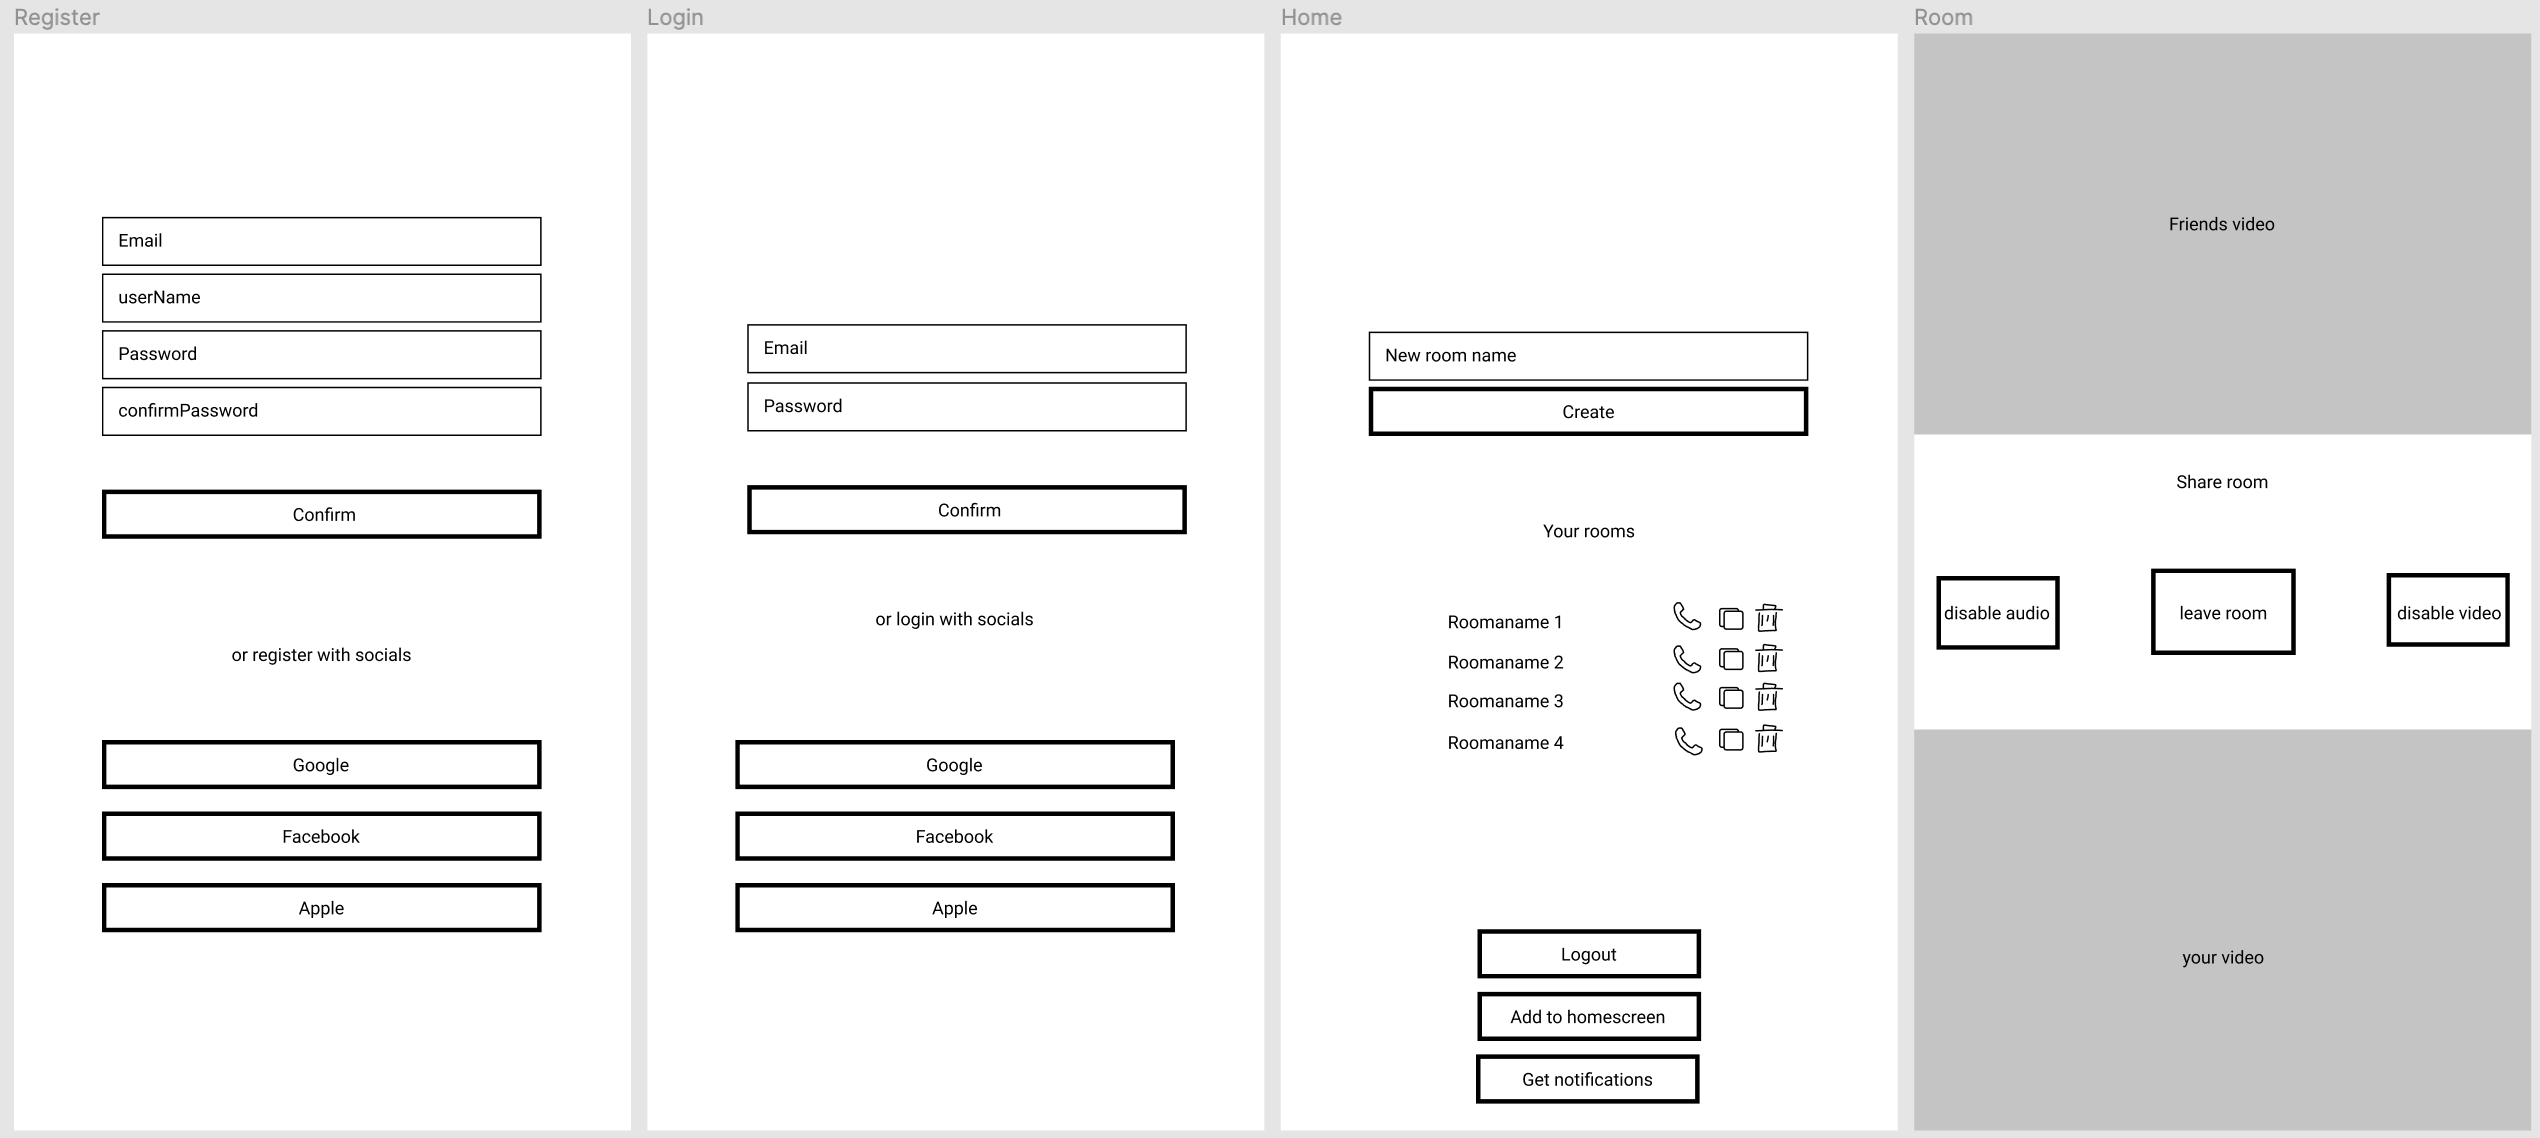
\includegraphics[width=140mm]{./img/mockup-poc.png}{}
				\caption{mockups in figma}
			\end{figure}
		
		
		\subsection{Prototype}
		
			Vervolgens werd er een klikbaar prototype gemaakt. In de dit prototype werd de stijl van de applicatie bepaald.
			
			Er werd gekozen om een eenvoudig design te implementeren met illustraties die van \href{https://undraw.co/}{unDraw} verkregen werden.
			
			\begin{figure}[H]
				\centering
				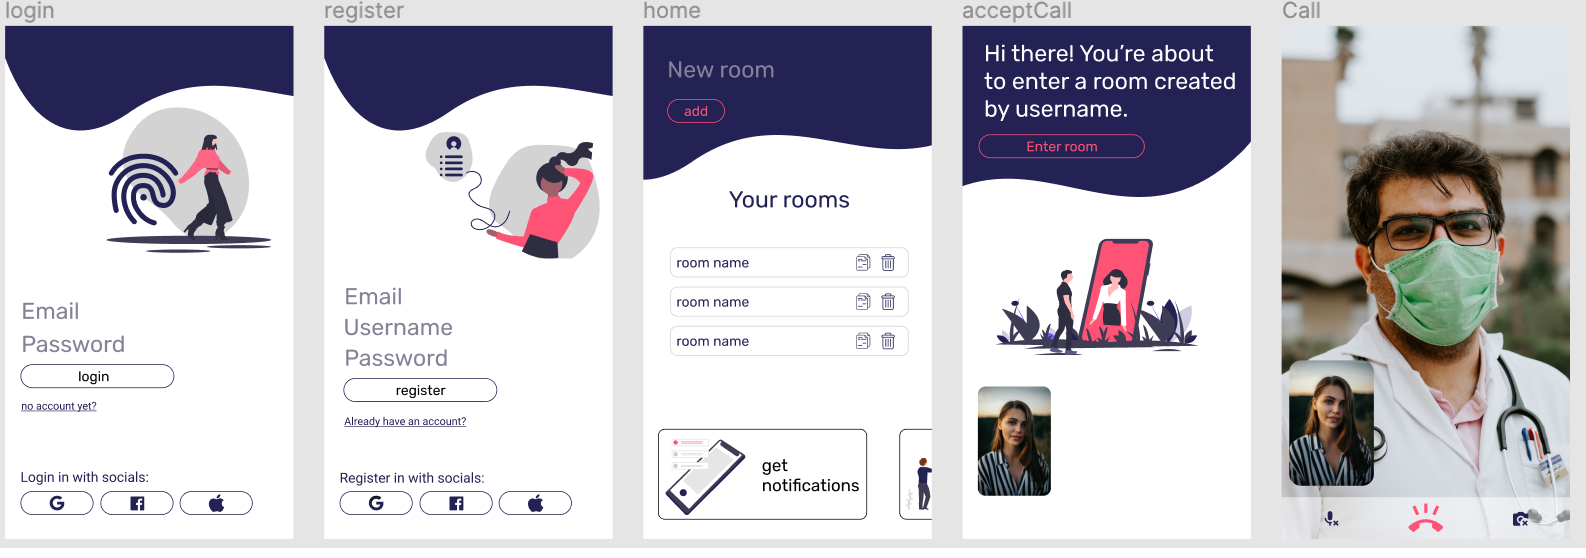
\includegraphics[width=140mm]{./img/prototype-poc.png}{}
				\caption{mockups in figma}
			\end{figure}
			
	
\section{Implementatie}
	Voor het ontwikkelen van de proof-of-concept werd er opnieuw gebruik van react.js voor de frontend. De backend werd ontwikkeld in node.js en als database werd firebase gebruikt.
	
	\subsection{Registreren service worker}
		
		In Hoofdstuk~\ref{ch:TransformerenNaarEenPWA} werd vermeld dat een standaard react applicatie al een service worker heeft die voor caching van statische bestanden zorgt. Deze service worker wordt gegenereerd tijdens het build proces door de library \href{https://github.com/goldhand/sw-precache-webpack-plugin}{sw-precache-webpack-plugin. }  
		\autocite{Mester2019}
		
		Door een service worker te genereren zorgt react ervoor dat een website heel eenvoudig is om statische bestanden te cachen en een website offline beschikbaar te maken.
		
		Deze strategie heeft echter een groot nadeel, de service worker die react genereerd kan kan niet worden aangepast door de ontwikkelaar. Als de applicatie een meer geavanceerde service worker nodig heeft, zal deze automatisch gegenereerde service worker moeten overschreven worden.
		
		Het artikel van Chinmaya Pati dat gepubliceerd werd op Medium beschrijft dit proces. \autocite{Pati2019}
		
	\subsection{A2HS}
	
		De applicatie voldoet aan alle criteria om geïnstalleerd te kunnen worden op toestellen. Echter zal de gebruiker geen standaard melding te zien krijgen om de applicatie te installeren.		
		
		Als de applicatie de gebruiker vraagt om de de applicatie toe te voegen aan het startscherm en de gebruiker staat dit niet toe, zal het beforeInstallPrompt nooit meer opnieuw opgeroepen worden. Deze melding kan dus maar 1 maal getoond worden.
		
		Om de kans te verhogen dat de gebruiker de applicatie toevoegt aan het startscherm zal deze melding enkel getoond worden als de gebruiker daar expliciet naar vraagt.
		\autocite{Mclachlan2020}
		
		Als de applicatie opstart zal het beforeInstallPrompt opgevangen worden en opgeslagen worden in de state. Door het standaard gedrag te overschrijven zal de melding nog niet getoond worden aan de gebruiker.
		\autocite{LePage2020b}
		
\begin{lstlisting}
window.addEventListener("beforeinstallprompt", (event) => {
	event.preventDefault();
	setPrompt(event);
}); 
\end{lstlisting}

		Vervolgens kan, als de gebruiker dit wenst, de melding toch getoond worden.
		
\begin{lstlisting}
const addToHome = () => {
	prompt.prompt();
};
\end{lstlisting}
	\subsection{Caching}
		\paragraph{Statish cachen}
			Statisch cachen is het cachen van bestanden die nodig zijn voor het opbouwen van de webapplicatie. Voorbeelden hiervan zijn foto's, style sheets, javascript bestanden, html bestanden, ...
			
			Op deze manier zal dus ook de application shell offline beschikbaar zijn.
			
			Door deze te cachen wordt de applicatie offline beschikbaar.
			
			In deze applicatie werd dit bereikt door workbox te gebruiken.
			
			In een eerste fase wordt het index.html bestand gecached.
\begin{lstlisting}
workbox.precaching.precacheAndRoute([
  {url: '/index.html', revision: '1'},
]);
\end{lstlisting}
		
			Workbox zal de functie 'precacheAndRoute' uitvoeren als de service worker geïnstalleerd wordt. De bestanden die worden meegeveven in de array zullen vanaf dat moment offline beschikbaar zijn.
			\autocite{Workbox2020a}
			
			Bestanden die hier toegoevoegd worden zullen geleverd worden aan de hand van de 'cache first' strategie. Dit wil zeggen dat dit bestand enkel aan de server gevraagd zal worden als het niet beschikbaar is in het cache geheugen.
			
			Een andere manier waarop statische caching kan gedaan worden is aan de van de 'registerRoute' die Workbow aanbiedt. 
			
\begin{lstlisting}
workbox.routing.registerRoute(
  /\.(?:js|css)$/,
  workbox.strategies.staleWhileRevalidate({
    cacheName: "static-resources",
    plugins: [
      new workbox.expiration.Plugin({
        maxEntries: 60,
        maxAgeSeconds: 20 * 24 * 60 * 60, // 20 Days
      }),
    ],
  })
);
\end{lstlisting}
			
			Aan de hand van een regular expression kunnen er bestanden gechached worden. In dit voorbeeld worden alle javascript en css bestanden offline beschikbaar gemaakt.
			
			In de voorbeeld wordt een andere strategie toegepast. de staleWhileRevalidate strategie houdt in dat eerst het gecachete bestand gebruikt wordt, vervolgens wordt het er een netwerkverzoek verstuurd om dit bestand op te halen van de server. Als deze bestanden niet volledig gelijk zijn, zal het gecachte bestand overschreven worden.
			\autocite{Workbox2020b}
			
			
					
		\paragraph{dynamisch cachen}
			Dynamisch cachen houdt in dat data die de gebruiker vraagt ook offline opgeslagen wordt. Dit zullen vaak requests van REST-API's zijn.
			
			In deze applicatie werd dynamisch cachen toegepast om de laatste versie van de rooms nog steeds te tonen aan de gebruiker, ookal als deze offline.
			
\begin{lstlisting}
workbox.routing.registerRoute(
  /.*(?:googleapis|)\.com.*$/,
  workbox.strategies.staleWhileRevalidate({
    cacheName: "firebase",
  })
);
\end{lstlisting}
		
		Opnieuw wordt er gebruik gemaakt van een regular expression om workbox duidelijk te maken welke request er offline beschikbaar moet zijn.

	\subsection{Authentication}
	
		https://www.smashingmagazine.com/2018/08/best-practices-for-mobile-form-design/
		
		Het invullen van van een form om een mobiel toestel is voor veel gebruikers een relatief grote inspanning.
		
		In het artikel van Nick Babich wordt de term "Interaction cost" gebruikt. De interaction cost is de som van alle cognitieve en fysieke inspanningen die een gebruiker moet doen om tot zijn doel te komen. Hoe lager de interaction cost hoe beter.
		
		Het invullen van formulieren met data heeft een hoge interaction cost. Er moet veel getypt worden (fysieke inspanning) en alles wat getypt moet worden moet correct zijn (cognitieve inspanning). het is dus belangrijk om de gebruiker hiervan te besparen.
		
		Dit kan gedaan worden door de gebruiker te laten registreren via een ander platform, hierbij moet er vaak helemaal niet, of veel minder getypt worden.
		
		Op deze applicatie kan de gebruiker zich aanmelden met Google en Facebook.
		
		Dit werd bereikt door gebruikt te maken van "Firebase authentication". Dit is een service die aangeboden wordt door Google.
		
		
\begin{lstlisting}
export const auth = firebase.auth();
const provider = new firebase.auth.GoogleAuthProvider();

export const authWithGoogle = () => {
return auth.signInWithPopup(provider)
};
\end{lstlisting}
	
		Deze code geeft alle relevante informatie terug die google over de gebruiker heeft. Dit bevat volgende eigenschappen:
		\begin{itemize}
			\item Voornaam
			\item Familienaam
			\item Volledige naam
			\item Email
			\item Profielfoto
			\item Voorkeurstaal
			\item ...
		\end{itemize} 
		
		Gelijkaardige code kan geschreven worden voor het aanmelden met andere platformen zoals:
		\begin{itemize}
			\item Twitter
			\item Github
			\item Apple
			\item Microsoft
			\item ...
		\end{itemize} 
		
	\subsection{Share API en Clipboard API}
	
		In de applicatie is het belangrijk om op een intuïtieve manier een link te kunnen delen naar een room. 
		Dit werd bekomen door de Share API te gebruiken.
		Op mobiele toestellen zal deze een native menu openen waar de gebruiker de link kan delen op via verschillende platformen.
		
		Echter bieden enkel chrome voor android en safari dit aan. Er kan er dus niet vanuit gegaan worden dat de gebruiker dit kan implementeren.

\begin{lstlisting}
 const shareData = {
      title: 'Join my room!',
      text: 'Click on the link and we can have a video chat ;-)',
      url: `https://videocall-pwa.netlify.app/visitroom/${owner}/${room}`,
    }
    navigator.share(shareData)
\end{lstlisting}

		\begin{figure}[H]
			\centering
			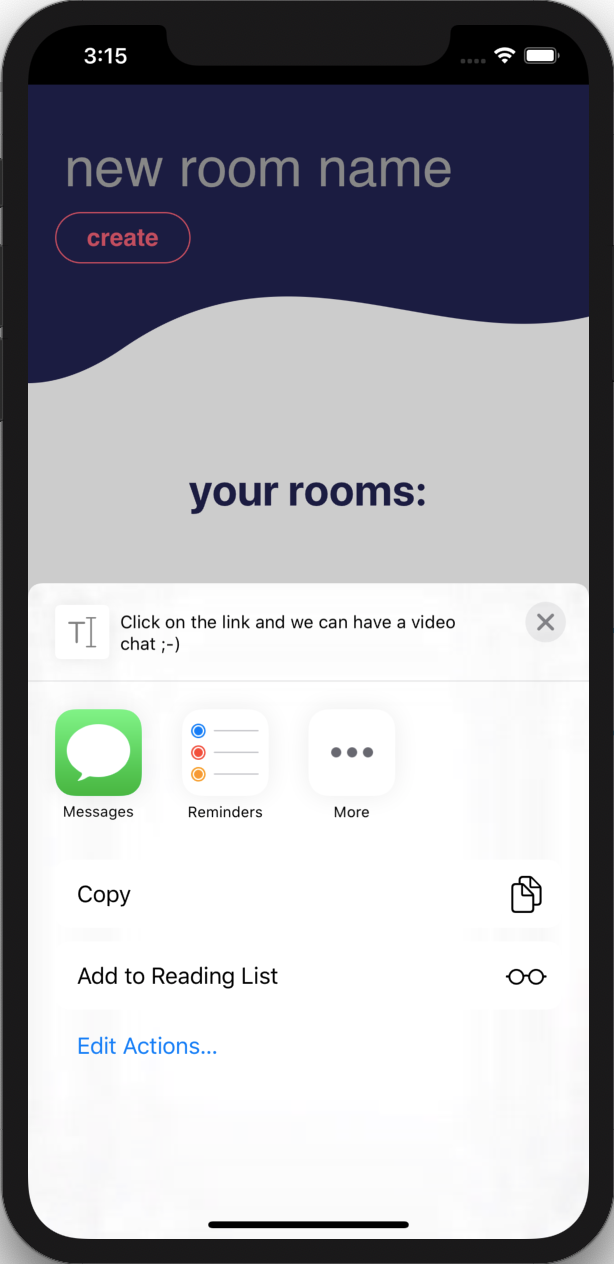
\includegraphics[width=35mm]{./img/share-ios}{}
			\caption{native share-menu op IOS}
		\end{figure}	
		\begin{figure}[H]
			\centering
			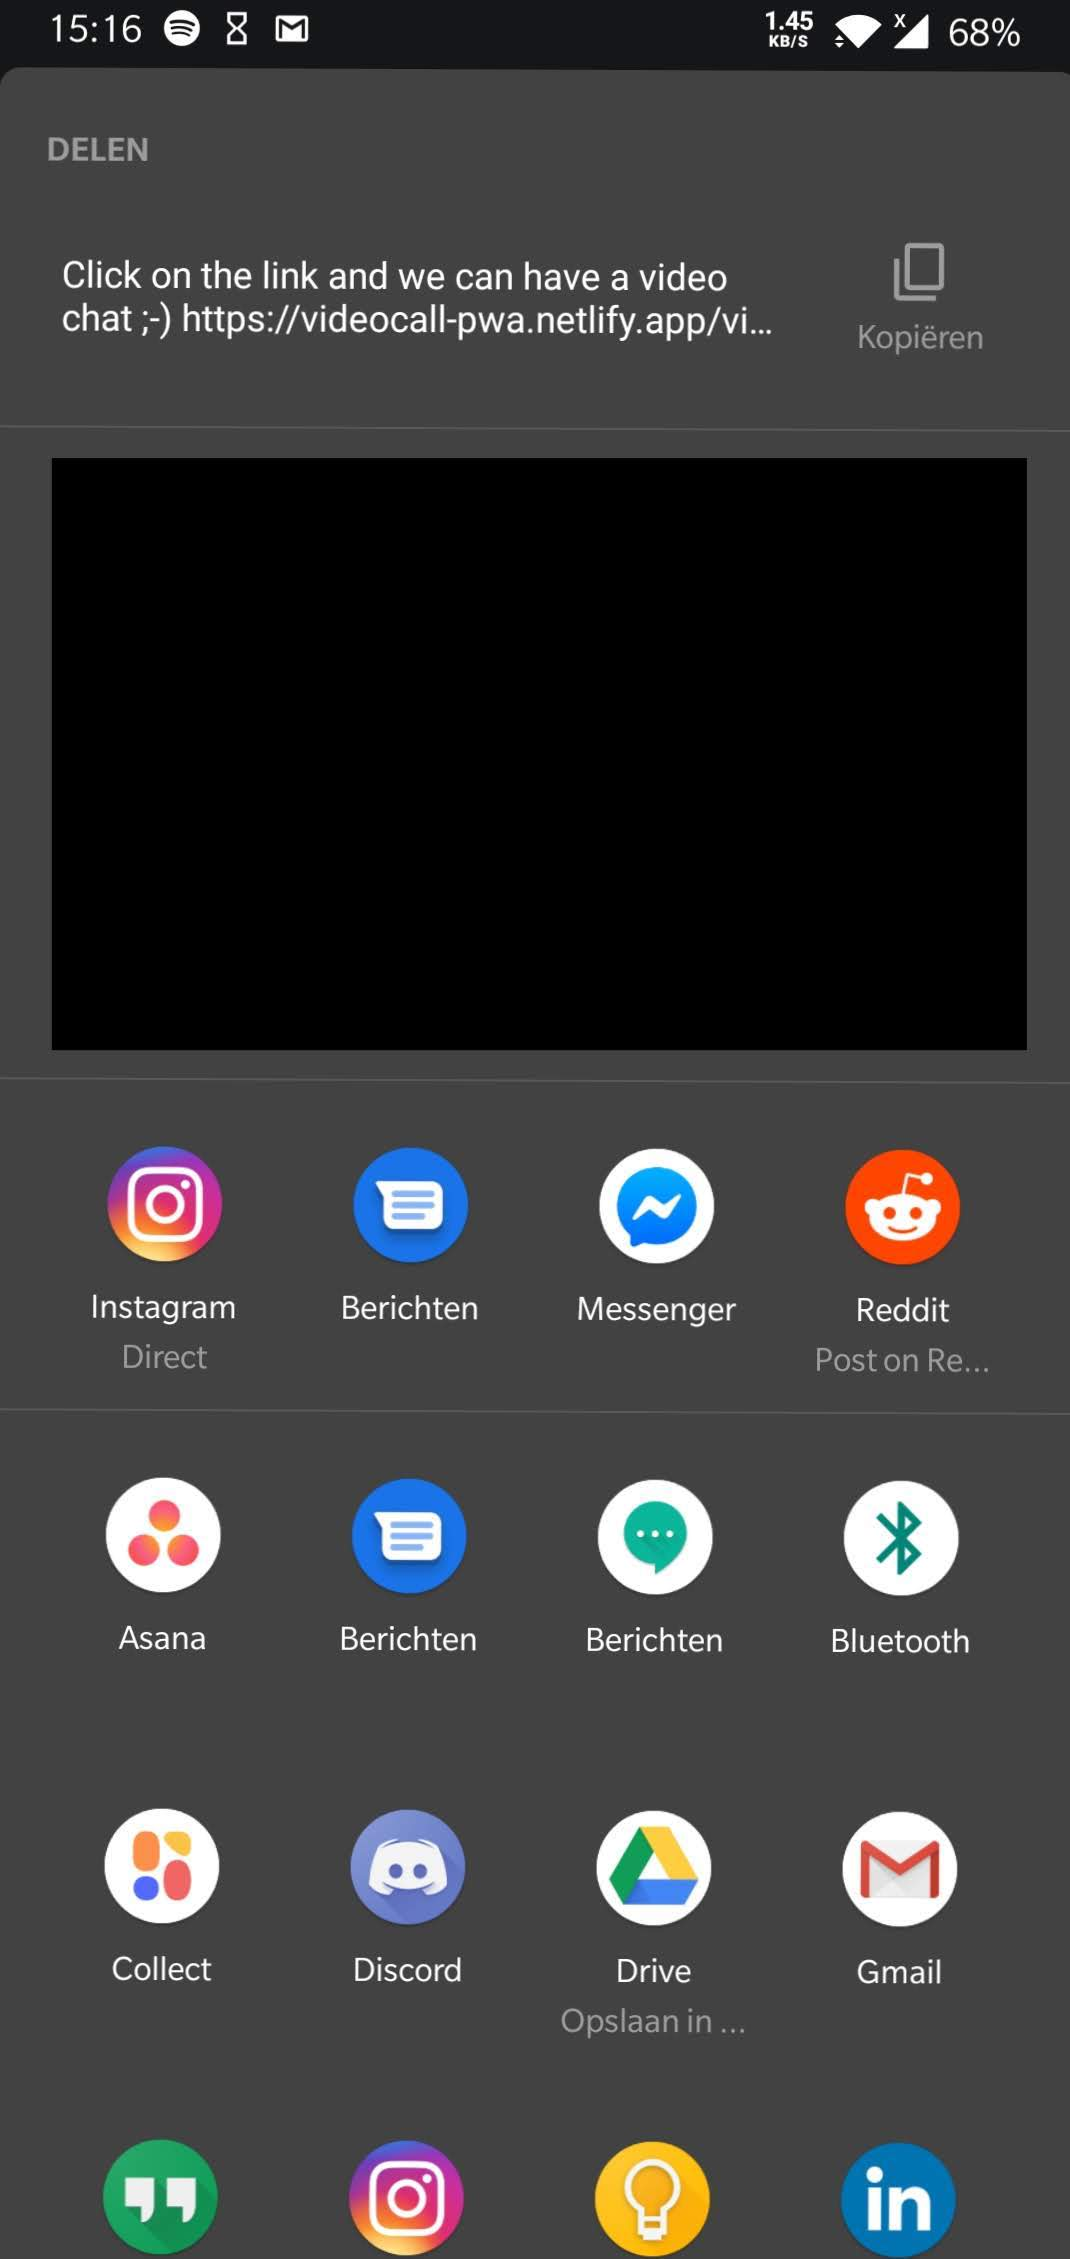
\includegraphics[width=35mm]{./img/share-android.jpg}{}
			\caption{native share menu op Android}
		\end{figure}

		Als de gebruiker een browser gebruikt die deze functie niet ondersteund, zal de clipboard API gebruikt worden.
	
		De clipboard API kan gebruikt worden om items in het klembord van de gebruiker te plaatsen of om het klembord uit te lezen.
		
		Deze web-API werd gebruikt om eenvoudig de link van de room te kunnen delen met een persoon die gecontacteerd zal worden.
		
		Volgende code zal de link genereren die de uitgenodigde persoon kan gebruiken en zal deze in het klembord van de gebruiker plaatsen.
		
		De eerste keer dat dit proces uitgevoerd wordt zal de gebruiker expliciet toestemming moeten geven om het klembord te mogen gebruiken.

\begin{lstlisting}
navigator.clipboard
  .writeText(`http://localhost:3000/visitroom/${roomownername}/${roomname}`)
  .then(() => {
    console.log("Text copied to clipboard");
    alert("coppied!! share the coppied link with somebody");
  });
};
\end{lstlisting}

		Bij deze feature werd er progressive enhancement toegepast. 
		In het beste geval wordt het native deel menu getoond, als dit niet beschikbaar is zal de link gekopiëerd worden in het klembord.
		Als ook dit niet beschikbaar is, of de gebruiker heeft geen toestemming gegeven zal er een boodschap getoond worden waar de gebruiker de link zelf kan kopiëren en delen.
		
\begin{lstlisting}
if('share' in navigator){
	// ... code voor het delen via een native menu ...
}
else{
	//... code voor het kopiëren van de link ...
	.catch(() => {
		//tonen van een boodscahp met de link die gedeeld moet worden
		swal(`you can share this link:
			https://videocall-pwa.netlify.app/visitroom/${owner}/${room}
		`);
	});
}
\end{lstlisting}


	\subsection{Push notificaties}
	
	https://web-push-book.gauntface.com/chapter-04/01-sending-messages-with-web-push-libraries/
	
	https://developers.google.com/web/fundamentals/push-notifications/subscribing-a-user
	
		Een van de grote voordelen van een PWA ten opzichte van een traditionele website is dat het push notificaties kan sturen naar de gebruiker.
		
		Er wordt aangeraden om de "web-push" library te gebruiken om push notificaties te implementeren
		
		https://developers.google.com/web/fundamentals/push-notifications/how-push-works
		
		\paragraph{Abbonneren op push notificaties}
			 De gebruiker moet expliciet toegang geven aan de webapplicatie om push notificaties te mogen gebruiken.
			 
\begin{lstlisting}
    const sw = await navigator.serviceWorker.ready;
    let pushSub = await sw.pushManager.subscribe({
          userVisibleOnly: true,
          applicationServerKey: 'public VAPID key
        })
\end{lstlisting}

			Dit stukje code zal een "subscription" teruggeven dat opgeslagen moet worden in de databank bij de gebruiker. deze "subscription" is uniek voor de gebruiker, de browser en het toestel.
			
			voorbeeld van een subscription:
	
\begin{lstlisting}
{
   "endpoint":"https://fcm.googleapis.com/fcm/send/fOkirMCCHhM:..."
   "expirationTime":null,
   "keys":{
      "p256dh":"BBwYLrPvd2IIAo4cWsJhXRD2g9aFyL1Q3K9cuWh_...",
      "auth":"0orvSHRZrMb3zP0yIpUAcg"
   }
}
\end{lstlisting}


		\paragraph{Backend}
			De backend moet in een eerste fase gebruikt worden om de VAPID keys te genereren.
			
			Vapid keys of application server keys zijn uniek voor de server
			
			Deze vapid keys zorgen ervoor dat de push services van de verschillende browsers weet van welke applicatie de notificaties afkomstig zijn. Hierdoor kan het ook de applicatie beveiligen en enkel deze server toestaan notificaties te sturen naar de applicatie.
			
			Elke browser heeft zijn eigen push service waar een applicatie server aan kan vragen om een notificiatie te sturen naar een bepaald toestel.
			
		
			Deze vapid keys kunnen in de applicatie server gegenereerd worden aan de hand van volgende code:
			
\begin{lstlisting}
console.log(push.generateVAPIDKeys)
\end{lstlisting}

			Dit zal een publieke en een private sleutel weergeven in de console. Deze moeten dan op een veilige plaats opgeslagen worden.
			
			Eens de server de Vapid keys heeft kan deze een notificatie verzenden.
			
\begin{lstlisting}
push.setVapidDetails(
    "mailto:mai",
    secrets.vapIdKeys.publicKey,
    secrets.vapIdKeys.privateKey
  );
  
 push.sendNotification( sub,  JSON.stringify({payload})
\end{lstlisting}

			Er moet ook een geldig email adres opgegeven worden. Dit email adres zal gebruikt worden door de push service als er problemen zijn met jouw applicatie.
			
			De push notificatie kan dan verzonden worden met eventueel extra informatie in de payload.
			
		\paragraph{Service worker}
		
			Op basis van de subscription die in de backend werd verzonden zal de service worker van de juiste gebruiker geactiveerd worden
			
			De service worker met een listener toevoegen waar eventuele push notificaties kunnen binnenkomen.
			
\begin{lstlisting}
self.addEventListener("push", function (e) {
	//handle notification
}
\end{lstlisting}
			
			Als de backend extra informatie heeft meegegeven kan deze uitgelezen worden.
\begin{lstlisting}
  const payload = JSON.parse(e.data.text())
\end{lstlisting}
			
			Vervolgens kan er een notificatie gevormd worden zoals eerder toegelicht
			
\begin{lstlisting}
options = {
      body: "Open the app and say hi!",
      icon: "images/example.png",
      vibrate: [300, 50, 100],
      data: {
        dateOfArrival: Date.now(),
        primaryKey: "2",
      },
    };

    e.waitUntil( self.registration.showNotification(`notification title`, options)
\end{lstlisting}
			
	\subsection{Local storage}
	
		https://developer.mozilla.org/en-US/docs/Web/API/Window/localStorage
		
		Om een ervaring aan te bieden zoals op native applicaties is het belangrijk om de gebruiker aangemeld te houden tussen sessies.
		
		Dit gebeurt aan de hand van local storage. Zolang de gebruiker het local storage niet manueel verwijdert zal dit blijven bestaan. 
		
		Als een gebruiker zich aanmeldt, wordt deze opgeslagen in het local storage.
		

	\subsection{Web RTC}
		https://webrtc.org/
		
		Web RTC is een verzameling van Web API's die real time commicatie op het web mogelijk maken. 
		
		In deze applicatie werd Web RTC gebruikt om:
		\begin{itemize}
			\item de camera van het toestel te gebruiken en een video-stream op het scherm te tonen.
			\item een peer-to-peer connectie op te zetten tussen twee gebruikers
			\item video tussen beide gebuikers te streamen
		\end{itemize} 
		
		Web RTC maakt gebruik van een peer-to-peer connectie tussen de twee gebruikers, tijdens het bellen is er dus geen server nodig. Echter, er is wel een server nodig om de connectie tussen beide tot stand te brengen.
		
		\paragraph{video-stream}
			De video-stream zal verkregen worden via het navigator object. Bij het opvragen van een video-stream zal de browser automatisch toestemming vragen aan de gebruiker als de camera en de microfoon gebruikt mag worden.
			
			Als de applicatie toestemming gekregen heeft wordt er een video-stream verkregen.
			Deze stream zal opgeslagen worden in de state van de applicatie en zal in een html-5 video element geplaatst worden.
		
\begin{lstlisting}
navigator.mediaDevices.getUserMedia({ 
		video: true,
		audio: true 
	}).then((stream) => {
		setYourVideoStream(stream);
		if (yourVideo.current) {
			yourVideo.current.srcObject = stream;
		}
	});
\end{lstlisting}


		\paragraph{peer-to-peer verbinding met streaming}
			Bij deze applicatie werd simple-peer gebruikt, dit is een abstractie van webRTC die het opzetten van peer-to-peer verbindingen eenvoudiger maakt.
			
			Voor beide gebruiker zal er een Peer object aangemaakt worden

\begin{lstlisting}
const peer = new Peer({
	initiator: true,
	trickle: false,
	stream: yourVideoStream,
});
\end{lstlisting}
			
			vervolgens zullen er listeners toegevoegd worden aan deze objecten die geactiveerd zullen worden op basis van het andere peer object
			
\begin{lstlisting}
peer.on("signal", (data) => {
	// code wordt uitgevoerd als er een andere peer aangemaakt wordt
});

peer.on("stream", (stream) => {
	// code wordt uitgevoerd als de andere peer start met het streamen van een video
});
\end{lstlisting}


	\subsection{Socket.io}
	
	%todo:	https://developer.mozilla.org/en-US/docs/Web/API/WebSockets_API
	
		Zoals eerder vermeld is er een server nodig om een peer-to-peer connectie tot stand te brengen.
		
		Deze backend werd geschreven in node.js en werd gehost op \href{https://glitch.com/}{glitch}.
		
		De library \href{https://socket.io/}{socket.io} werd gebruikt websocktets te implementeren. Websockets zorgen ervoor dat een server met de frontend kan cummuniceren zonder dat deze er expliciet om vragen. 
		
		In traditionele applicaties krijgt de frontend enkel data als hij hier een request voor stuurt naar de backend, bij websockets kan de backend de frontend met data voorzien in real time.
		
		Deze real-time communicatie is nodig voor het opzetten van een peer-to-peer connectie.
		
		De backend zal de frontend informeren als er een gebruiker in een room komt, vervolgens kan er een peer-to-peer connectie opgezet worden.
		
		Zowel de frontend als de backend kunnen een event sturen en naar events luisteren. Op deze manier wordt er gecomuniceerd. 	
		
			
	\subsection{Masked icons}
	
		Het startscherm van android toestellen kan in veel verschillende vormen komen. De producent van een android toestel kan zelf een thema ontwikkelen voor het startscherm.
		
		In verschillende thema's zullen de icoontjes er anders uitzien, in sommige thema's zullen ze rond zijn, in andere vierkant met afgeronde hoeken. 
		
		Als het icoontje niet geoptimaliseerd wordt, zal Android er steed voor zorgen dat het icoontje volledig zichtbaar is. Indien nodig zal er een achtergrond toegevoegd worden.
		
	
		%todo: image van niet gemaskte iconen
		
		Door ervoor te zorgen dat alle belangrijke elementen va het icoon binnne een 'safe zone' vallen, en een extra property toe te voegen in het app manifest kan dit opgelost worden.
		
\begin{lstlisting}
"purpose": "any maskable" 
\end{lstlisting}
		% todo: image van wel gemaskte iconen
		%todo: imag van vid call icoon	
		
		

\section{De Applicatie}
	%todo: screenshots toevoegen
	\subsection{Authenticatie}
		De gebruiker kan zich registreren aan de hand van een email en wachtwoord combinatie. Er is ook een optie om zicht aan te melden aan de hand van google en facebook.
		
		
	\subsection{Home}
		Dit is het scherm waar de gebruiker zal terechtkomen als hij is aangemeld. 
		Op dit scherm kan de gebruiker zijn rooms beheren, hij kan nieuwe rooms aanmaken, rooms verwijderen en rooms delen.
		
		Onderaan de pagina is er een horizontale scroll, in deze lijst kan de gebruiker volgende opties:
		\begin{itemize}
			\item De applictie installeren en toevoegen aan het startscherm
			\item Notificaties aan zetten 
			\item Afmelden
		\end{itemize}
		
	\subsection{Wachtschermen}
		Als er slechts 1 persoon is in de room zal de gebruiker op dit scherm terechtkomen. 
		
		De eigenaar van de room heeft een optie om de room te delen. 
		
		Als een bezoeker in de room komt, zal de eigenaar een melding krijgen dat er iemand in zijn room is. Door op de notificatie te klikken gaat de eigenaar direct naar de room.
						
		Als beide gebruikers aanwezig zijn, zal de bezoeker de optie krijgen om het gesprek te starten.
		
	\subsection{Room}
		In dit scherm kunnen de gebruikers een conversatie hebben. 
		
		Er is een optie om het gesprek te beëindigen, het geluid uit te schakelen en de video stream uit te schakelen.
		
	\subsection{Notificaties}
		Op dit scherm kan de administrator van de applicatie een zelf gekozen notificatie versturen naar alle gebruikers die hun goedkeuring hebben gegeven om notificaties te ontvangen.
		

\section{Conclusie}
	
	Al de vooropgestelde requirements kunnen bereikt worden door een PWA te implementeren. 
	
	Native features zoals camera, microfoon, delen, notificatie zijn relatief eenvoudig te implementeren in een webapplicatie.
	
	Echter, iets wat minder meetbaar is, de applicatie voelt niet aan als een native applicatie.
	
	Het is niet eenvoudig om consistent een goeie ervaring te bieden met één codebase voor alle platformen die ondersteund worden. 
	
	Er werd beslist om de maximale hoogte van de applicatie vast te zetten op 100vh,  op deze manier is het in princiep onmogelijk om een scroll van de volledige pagina te hebben. 
	
	dit werkte goed op een desktop browser maar gaf problemen op mobiele toestellen.
	
	Op Android bijvoorbeeld maakt de adresbalk geen deel uit van de viewport. Hierdoor was er dus wel een scroll van enkele centimeters aanwezig als de applicatie bezocht werd in de browser. Dit probleem wordt opgelost als de applicatie geïnstalleerd wordt, dan is er geen adresbalk aanwezig.
	
	%todo: screenshot van inconsitentie
	
	
	
	
	
			
		